\documentclass[tikz,border=6pt]{standalone}
\usetikzlibrary{arrows.meta,positioning,calc,fit}
\makeatletter
\AtBeginDocument{\global\let\pgf@selectfontorig\relax}
\makeatother

\tikzset{
  state/.style={
    draw=black,
    rounded corners=4pt,
    very thick,
    fill=white,
    minimum width=8.5mm,
    minimum height=7mm,
    align=center,
    inner sep=1.6pt,
    font=\scriptsize
  },
  edge/.style={-Latex, thick, shorten >=2pt, shorten <=2pt},
  labelbox/.style={fill=white, inner sep=1.2pt, font=\scriptsize},
  panel/.style={draw=gray!70, rounded corners=6pt, very thick},
  title/.style={fill=white, inner sep=1.5pt, font=\itshape\large}
}

\newcommand{\componentpanel}[4]{
  \draw[panel] #1 rectangle #2;
  \node[title, anchor=north west] at #3 {$#4$};
}

\begin{document}
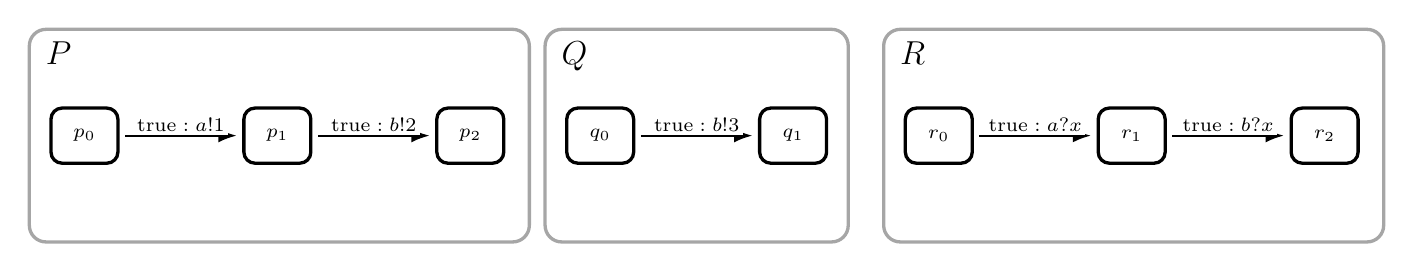
\begin{tikzpicture}[scale=1, transform shape]

  \begin{scope}[shift={(0,0)}]
    \node[state] (p0) at (0,0) {$p_0$};
    \node[state] (p1) at (2.45,0) {$p_1$};
    \node[state] (p2) at (4.9,0) {$p_2$};
    \draw[edge] (p0) -- node[labelbox, above] {$\mathrm{true}:a!1$} (p1);
    \draw[edge] (p1) -- node[labelbox, above] {$\mathrm{true}:b!2$} (p2);
    \componentpanel{(-0.7,-1.35)}{(5.65,1.35)}{(-0.55,1.25)}{P}
  \end{scope}

  \begin{scope}[shift={(6.55,0)}]
    \node[state] (q0) at (0,0) {$q_0$};
    \node[state] (q1) at (2.45,0) {$q_1$};
    \draw[edge] (q0) -- node[labelbox, above] {$\mathrm{true}:b!3$} (q1);
    \componentpanel{(-0.7,-1.35)}{(3.15,1.35)}{(-0.55,1.25)}{Q}
  \end{scope}

  \begin{scope}[shift={(10.85,0)}]
    \node[state] (r0) at (0,0) {$r_0$};
    \node[state] (r1) at (2.45,0) {$r_1$};
    \node[state] (r2) at (4.9,0) {$r_2$};
    \draw[edge] (r0) -- node[labelbox, above] {$\mathrm{true}:a?x$} (r1);
    \draw[edge] (r1) -- node[labelbox, above] {$\mathrm{true}:b?x$} (r2);
    \componentpanel{(-0.7,-1.35)}{(5.65,1.35)}{(-0.55,1.25)}{R}
  \end{scope}

\end{tikzpicture}
\end{document}
